%!TeX root=../tese.tex
%(dica para o editor de texto: este arquivo é parte de um documento maior)
% para saber mais: https://tex.stackexchange.com/q/78101/183146

\chapter{Perceptron multi-camadas}
\label{cap:perceptron}

Neste capítulo é descrita a implementação e funcionamento de uma versão do algoritmo \eng{perceptron}, feito a partir de um núcleo básico disponibilizado no livro de Kopec \citep{classic}, e a partir do qual foram feitas modificações e criação de novos métodos de treinamento, de validação e de avaliação do treinamento.

O perceptron aqui implementado tem o objetivo de ser utilizado muito mais para fins didáticos do que práticos e pode ser usado para tarefas de aprendizagem contanto que sejam problemas que envolvam bases de dados de tamanho pequeno ou mediano, e neste capítulo é apresentadao um caso de uso para um problema de classificação de dados.

Na última parte desse capítulo é exibida uma biblioteca de \eng{machine learning} utilizada nas aplicações reais de \eng{deep learning} de redes neurais, muito mais avançada, com muitos outros recursos que vão além do escopo que esta versão simples do \emph{perceptron} é capaz de lidar. Esta será a biblioteca de redes neurais que será utilizada nas partes práticas deste trabalho.

\section{Matemática do algoritmo de retropropagação}

Para a aprendizagem supervisionada foi utilizado o algoritmo de retropropagação (\eng{retropropagation}), que consiste na minimização de uma função de custos, a partir do gradiente, ou seja, da derivada desta função de custos, neste caso o erro quadrático médio, conforme foi definido no capítulo anterior.

De acordo com Kopec \citep{classic}, o perceptron consiste de uma rede cujo sinal, ou seja, os dados, se propagam em uma só direção, da camada de entrada para a camada de saída, passando pelas camadas ocultas uma a uma, e por isso o nome de rede \eng{feedforward} ao perceptron. Por sua vez, o erro que determinamos na camada final propaga-se no caminho inverso, sendo distribuídas correções da saída para a entrada, afetando aqueles neurônios que foram mais responsáveis pelo erro total. Por isso o nome de retropropagação.

Estendendo as definições já usadas no capítulo anterior, segue a derivação matemática do algoritmo de retropropagação. Como ficará claro mais à frente, podemos derivar as contas para apenas um neurônio por camada sem perda de generalidade. Dessa forma, se temos uma rede com $L$ camadas, o erro quadrático para um neurônio da camada de saída (a camada $L$) será:
\[
C_0 = (a^{(L)} - y)^2
\]
onde $y$ é a saída esperada, e $a^{(L)}$ é a saída de um neurônio da camada de saída.

Temos que $C_0$ é uma função de $a^{(L)}$, uma vez que $y$ é um valor fixo conhecido. Por sua vez, temos que de modo geral a saída de um neurônio é uma função do tipo:
\[
a^{(L)} = \sigma(w^{(L)}~a^{(L-1)} + b^{(L)})
\]
onde escrevemos $a^{(L-1)}$ é a saída do neurônio da camada anterior, $w^{(L)}$ é o \defi{peso} atribuido a essa saída, o que seria o parâmetro angular $A$ na Figura \ref{fig:neuronio}, e $b^{(L)}$ é o chamado \defi{viés} desse neurônio, análogo ao parâmetro linear de uma reta. Por fim temos a \defi{função de ativação} que escrevemos como $\sigma$ que é aplicada à essa equação linear.

Nota-se que internamente à função de ativação, um neurônio se comporta como uma transformação linear dos neurônios da camada anterior. Caso tivéssemos $n$ neurônios na camada anterior à de saída, teríamos então $n$ pesos, denotados com índice $i$ dessa forma: $\{ w_i^{(L)} \}_{i=1}^n$. Cabe assim à função de ativação, dar o comportamento não-linear à rede perceptron.

Como o objetivo é minimizar $C_0$, temos que calcular a influência dos pesos e dos viéses nesse custo. Já sabemos que isso será obtido com o gradiente, isto é, a derivada dessa função em relação a esses parâmetros que, são os únicos que podemos otimizar. De forma mais clara, temos que no início do treinamento da rede, atribuímos valores aleatórios aos pesos e aos viéses, e então executamos o \eng{feedforward}, de forma que a rede irá calcular sequencialmente os valores de saída em todas as suas camadas, obtidos a partir dos dados de entrada, que serão fixos, e desses parâmetros inicialmente aleatórios. A partir daí, poderemos otimizar esses parâmetros, exatamente da forma que estamos construindo.

O cálculo dessas derivadas é feito segundo a regra da cadeia, e adicionalmente iremos denotar a transformação linear interna à função de ativação por $z^{(L)} = w^{(L)}~a^{(L-1)} + b^{(L)}$, de forma que $a^{(L)} = \sigma(z^{(L)})$. Assim, ficamos com as derivadas para a camada de saída:

\begin{equation}\label{retro:1}
\frac{\del C_0}{\del w^{(L)}} = \frac{\del z^{(L)}}{\del w^{(L)}} \frac{\del a^{(L)}}{\del z^{(L)}} \frac{\del C_0}{\del a^{(L)}}
\end{equation}

\begin{equation}\label{retro:2}
\frac{\del C_0}{\del b^{(L)}} = \frac{\del z^{(L)}}{\del b^{(L)}} \frac{\del a^{(L)}}{\del z^{(L)}} \frac{\del C_0}{\del a^{(L)}}
\end{equation}

Para a camada de saída, podemos calcular diretamente cada termo dessas derivadas:

\begin{equation}\label{retro:4}
\frac{\del C_0}{\del a^{(L)}} = 2(a^{(L)} - y) ~\propto~ (a^{(L)} - y)
\end{equation}

\begin{equation}\label{retro:5}
\frac{\del a^{(L)}}{\del z^{(L)}} = \sigma^{'}(z^{(L)})
\end{equation}

\begin{equation}\label{retro:6}
\frac{\del z^{(L)}}{\del w^{(L)}} = a^{(L-1)}
\end{equation}

\begin{equation}\label{retro:7}
\frac{\del z^{(L)}}{\del b^{(L)}} = 1
\end{equation}

O que resulta, fazendo todas as substituições, em:

\begin{equation}\label{retro:10}
\frac{\del C_0}{\del w^{(L)}} = a^{(L-1)}~ \sigma^{'}(z^{(L)})~ (a^{(L)} - y)
\end{equation}

\begin{equation}\label{retro:11}
\frac{\del C_0}{\del b^{(L)}} = \sigma^{'}(z^{(L)})~ (a^{(L)} - y)
\end{equation}

Na equação \ref{retro:4} ocultamos o termo constante $2$ sob um símbolo de proporção, que a seguir iremos também ocultar, uma vez que usaremos o algoritmo do gradiente descendente, e assim, em seu lugar, e na verdade, todas as derivadas aqui mostradas serão multiplicadas pelo termo $\eta$, a \defi{taxa de aprendizagem}, conforme explicado no capítulo anterior. 

Analogamente, podemos pensar numa forma de fazer esses cálculos para as camadas ocultas. A princípio, podemos calcular:

\begin{equation}\label{retro:3}
\frac{\del C_0}{\del a^{(L-1)}} = \frac{\del z^{(L)}}{\del a^{(L-1)}} \frac{\del a^{(L)}}{\del z^{(L)}} \frac{\del C_0}{\del a^{(L)}}
\end{equation}

Usando o fato de que:

\begin{equation}\label{retro:8}
\frac{\del z^{(L)}}{\del a^{(L-1)}} = w^{(L)}
\end{equation}

Agora, seja a $i$-ésima camada oculta tal que $1 < i < L$, se observarmos a equação \ref{retro:3}, e fizermos $i = L-1$, usando a equação \ref{retro:8}, ficamos com:

\begin{equation}\label{retro:9}
\frac{\del C_0}{\del a^{(i)}} = w^{(i+1)} \frac{\del a^{(i+1)}}{\del z^{(i+1)}} \frac{\del C_0}{\del a^{(i+1)}}
\end{equation}

Podemos observar que há um mesmo termo duplo que aparece tanto nas equações \ref{retro:1} e \ref{retro:2} quanto na equação \ref{retro:9} acima, de forma que apenas o índice da camada é diferente. Para simplificar podemos nomear esse termo de \emph{delta da camada $i$}:

\begin{equation}\label{retro:12}
\Delta^{(i)} = \dfrac{\del a^{(i)}}{\del z^{(i)}} \dfrac{\del C_0}{\del a^{(i)}}
\end{equation}

Simplificando todas as demais expressões usando essa definição, ficamos com:

\begin{equation}\label{retro:13}
\frac{\del C_0}{\del w^{(i)}} = a^{(i-1)} \Delta^{(i)}
\end{equation}

\begin{equation}\label{retro:14}
\frac{\del C_0}{\del b^{(i)}} = \Delta^{(i)}
\end{equation}

Como vemos, as derivadas que precisamos todas dependem desse termo $\Delta$, que por sua vez depende do cálculo do termo $\dfrac{\del C_0}{\del a^{(i)}}$ que será calculado de 2 formas distintas:

\[ \dfrac{\del C_0}{\del a^{(i)}} = w^{(i+1)}~ \Delta^{(i+1)}  \;\;\Rightarrow \]
\begin{equation}\label{retro:15}
\Delta^{(i)} = \sigma^{'}(z^{(i)})~ w^{(i+1)}~ \Delta^{(i+1)}
\end{equation}
para as camadas ocultas.


\[ \dfrac{\del C_0}{\del a^{(L)}} = (y - a^{(L)}) \;\;\Rightarrow \]
\begin{equation}\label{retro:16}
\Delta^{(L)} = \sigma^{'}(z^{(L)})~ (y - a^{(L)})
\end{equation}
para a camada de saída.

Percebe-se a natureza recursiva do algoritmo, onde o caso base é calculado na camada de saída, e que o cálculo vai propagando-se para as camadas ocultas, em direção à camada de entrada. Por essa mesma razão, pudemos derivar as contas para uma camada, e no fim elas estão prontas pra serem implementadas para qualquer número de camadas ocultas. 

Outro fato útil é que a expressão interna do neurônio é uma transformação linear, assim as contas podem ser facilmente ajustadas para o caso geral em que há $n_i$ neurônios em dada camada $i$ da rede, conforme já explicado, e que será detalhado diretamente nos trechos de código que serão mostrados a seguir na implementação propriamente dita.

\section{Implementação do algoritmo de retropropagação}

A implementação seguiu uma estrutura orientada a objetos, voltemos então à representação visual da rede perceptron, a partir da imagem \ref{fig:estrutura_rn}. Cada círculo representa um neurônio, cada coluna vertical de neurônios é uma camada da rede, uma das camadas, a camada oculta nesse caso, está destacada em roxo na imagem. As setas representam as conexões entre as camadas de neurônios, cada neurônio de uma camada está ligado a todos os neurônios da camada anterior, o sentido dessa conexão é da esquerda pra direita, o que indica o processo de \eng{feedforward} da rede.

\begin{figure}[htb]
\centering
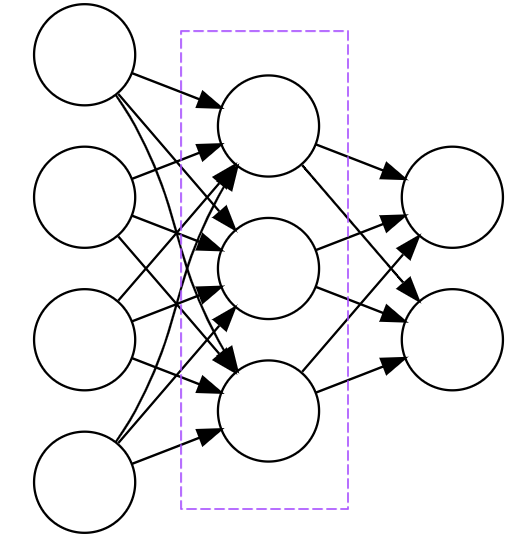
\includegraphics[width=6cm]{figuras/estrutura_rn}
\caption{Visão estrutural da rede perceptron. A linha tracejada destaca uma das camadas da rede.}
\label{fig:estrutura_rn}
\end{figure}

A implementação do perceptron deste trabalho teve como base a implementação feita por Kopec \citep{classic}, a partir da qual foram adicionados outros recursos, como o viés dos neurônios, não presentes na implementação de Kopec, como o uso da biblioteca \emph{Numpy} para o uso de seus métodos mais eficientes para lidar com listas de números de ponto flutuante. Além dessa base, também estão implementadas várias outras classes, que serão explicadas de modo mais geral.

\subsection{O neurônio}

O primeiro passo é implementar a classe \emph{Neuron} para representar cada neurônio. Esta é uma classe de entidade bem simples, contendo apenas um construtor, e o método \eng{output} que recebe os valores de entrada para esse neurônio e faz o cálculo da transformação linear e a seguir aplica e retorna o valor da função de ativação utilizada, que é passada como parâmetro ao construtor da classe. A listagem \ref{lst:neuron} abaixo mostra este método, em conjunto com o construtor da classe.

\begin{scriptsize}
\estiloR
\begin{lstlisting}[caption={Trecho da classe Neuron}, label={lst:neuron}, escapeinside={\%}]
class Neuron:
    def __init__(self, weights, bias, learning_rate, ativacao, der_ativacao):
        '''(list[float], float, float, Callable, Callable) -> None'''
        ...

    def output(self, inputs):
        '''(list[float]) -> float'''
        self.output_cache = np.dot(inputs, self.weights) + self.bias
        return self.ativacao(self.output_cache)
\end{lstlisting}
\end{scriptsize}

A função \emph{np.dot} da biblioteca \emph{Numpy} é utilizada para calcular o produto escalar entre os valores de entrada e os pesos desse neurônio. O valor da transformação linear é armazenado num atributo de classe antes da aplicação da função de ativação, pois será utilizado mais à frente durante o treinamento da rede.

\subsection{A função de ativação}

A função de ativação possui o papel de ativar ou não a saída de um neurônio, conforme visto no capítulo anterior, e a forma com que essa ativação ocorre é definida pela função utilizada. Aqui o termo \emph{ativar} significa que a função irá retornar um valor mais próximo de $1$ enquanto que uma não-ativação retornará um valor mais próximo de $0$. Essa é uma restrição para a função de ativação para a camada de saída, que será sempre da forma:

\[ f: \mathbb{R} \rightarrow [0, 1] \]

No caso do neurônio biológico, quando dizemos que ele ativa/transmite ou não o sinal elétrico que chegou até ele, é como se ele \emph{retornasse} apenas $0$ ou $1$. De fato, poderíamos até usar uma função similar a essa em alguma camada de nossa rede artificial, e este tipo de função escada tem a seguinte definição:

\[
f(x) = 
\left\{
\begin{array}{lcr}
1 & \text{se} & x \geq 0\\
0 & \text{se} & x < 0
\end{array}
\right.
\]

A utilização dessa função de ativação, conforme nos diz Grus \citep{data}, faria com que um neurônio fizesse simplesmente a distinção entre espaços separados pelo hiperplano de pontos tal que $ <w.x> + b = 0$, ou seja, o hiperplano definido pelos pontos de entrada cuja transformação linear resultasse em zero.

Esta função é claramente não contínua e portanto não diferenciável, e precisamos de uma função de ativação que o seja, uma vez que algumas das equações da otimização que calculamos anteriormente, dependem da expressão de sua derivada. É por essa razão, que Grus \citep{data} nos explica que passou-se a considerar uma aproximação suave da função escada, essa aproximação é a função \eng{sigmoid}:

\[
\sigma(x) = \frac{1}{1 + e^{-x}}
\]

Ela retorna valores somente no intervalo $[0, 1]$, igualmente à função escada, sua inspiração. Essa característica, no entanto, não é uma restrição para as camadas ocultas da mesma forma que é para a camada de saída, uma vez apenas a camada de saída será comparada com valores esperados no intervalo $[0, 1]$. A sua derivada pode ser facilmente calculada, e sua expressão simplifica-se como:

\[
\sigma^{'}(x) = \sigma(x)(1-\sigma(x))
\]

Podemos comparar o comportamento dessas funções de ativação no gráfico presente na imagem \ref{fig:ativacao} abaixo. A seguir, na listagem \ref{lst:ativacao}, um trecho do script \texttt{util.py} com a implementação da função \eng{sigmoid} e de sua derivada.

\newpage

\begin{figure}[htb]
\centering
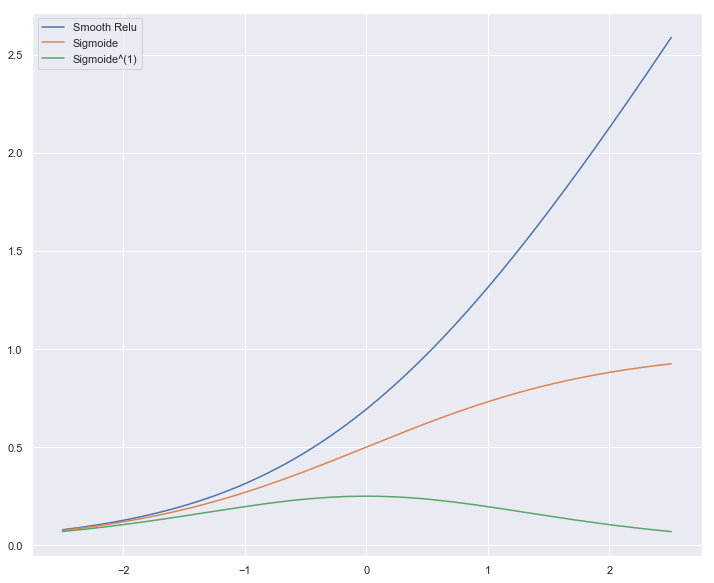
\includegraphics[width=12cm]{figuras/ativacao}
\caption{Comparação entre as funções de ativação do tipo escada e a \eng{sigmoid}.}
\label{fig:ativacao}
\end{figure}

\begin{scriptsize}
\estiloR
\begin{lstlisting}[caption={Trecho do script util.py}, label={lst:ativacao}, escapeinside={\%}]
def sigmoid(x):
    '''(float) -> float'''
    return 1.0 / (1.0 + np.exp(-x))

def der_sigmoid(x):
    '''(float) -> float'''
    sig = sigmoid(x)
    return sig * (1 - sig)
\end{lstlisting}
\end{scriptsize}

Com a popularização das redes neurais, várias outras funções de ativação foram criadas para ativarem as camadas ocultas do treinamento, devido aos problemas que podem acontecer ao se utilizar função \eng{sigmoid}. Podemos identificar um desses problemas analisando seu gráfico. Vemos que ela se aproxima de $1$, que é a ativação máxima, rapidamente a partir de $x > 4$, e aproxima-se simetricamente de zero com valores a partir de $x < -4$. 

Como o método do gradiente tenta ajustar os valores dos pesos a partir dos valores de saída e esses ajustes dependem da derivada da função de ativação, temos que levar em conta o comportamento da derivada da função \eng{sigmoid}, o qual podemos observar a partir de seu gráfico na figura \ref{fig:der_sigm}.

\begin{figure}[htb]
\centering
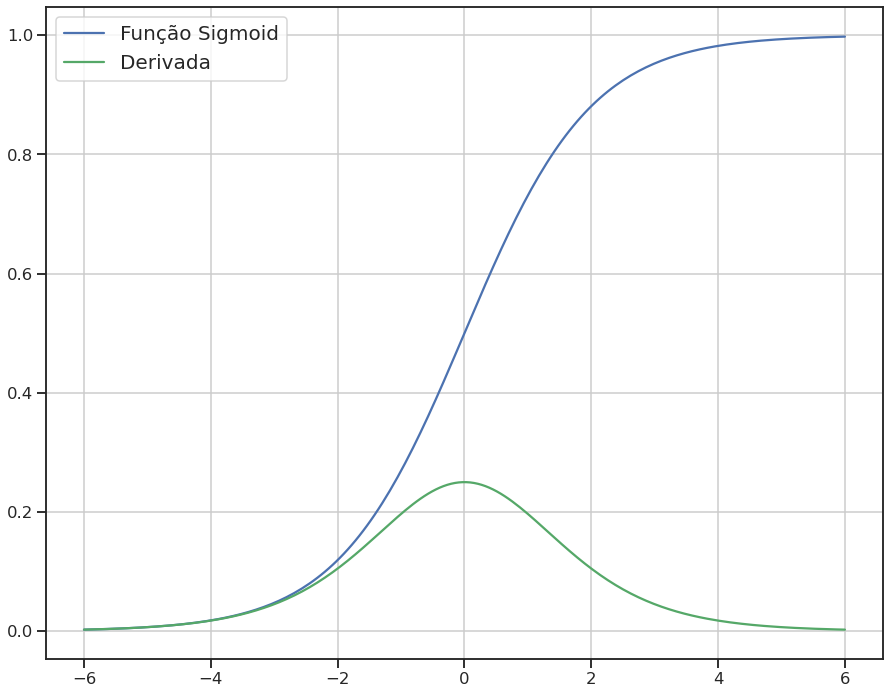
\includegraphics[width=12cm]{figuras/der_sigm}
\caption{Gráficos da função \eng{sigmoid} e sua derivada.}
\label{fig:der_sigm}
\end{figure}

Como podemos ver, a derivada retorna valores sempre menores do que $1$, e além disso aproxima-se de $0$ tão rapidamente quanto a \eng{sigmoid} aproxima-se de $1$. Isso faz com que atualizações para valores de saída que já estão muito altos não sejam efetivos para diminuí-los, pois justamente nessa região a derivada está muito próxima de $0$. Essa é a desvantagem da função \eng{sigmoid}.

Um problema relacionado a este é que se a regra da cadeia em \ref{retro:1} e \ref{retro:2}, com as derivadas da função de ativação dadas em \ref{retro:5} multiplicadas através das várias camadas, pode resultar num número muito grande, se todas as derivadas resultarem em valores maiores do que $0$, ou resultar num número muito próximo de $0$ se todas as derivadas forem menores do que $0$. Isto faz com que atualizações dadas pelo gradiente sejam instáveis. Este é o problema descrito por Matheus Facure \citep{matheus_2} e nomeado como problema do gradiente explodindo/desvanecendo. (\eng{exploding/vanishing gradient problem}).

Assim, conforme nos diz Facure \citep{matheus}, a utilização da função \eng{sigmoid} não é mais recomendada em problemas que envolvam de redes neurais maiores, sendo bem comum o problema do gradiente explodindo, já que a derivada é sempre maior do que $0$. Porém, ele também diz que alguns modelos probabilísticos de variáveis binárias, modelagem de problemas biológicos onde ela é uma aproximação mais plausível da ativação elétrica-biológica, e também alguns modelos não supervisionados de redes tem restrições que fazem com que seja não só desejável como também necessário o uso da função \eng{sigmoid}.

A próxima função de ativação é a o tangente hiperbólico $\tanh(x)$, ela é similar à \eng{sigmoid} e pode ser escrita em função dela. Ela retorna valores no intervalo $[-1, 1]$ mas sua derivada retorna valores mais próximos de $1$, chegando ao valor máximo de $1$ quando $x = 0$. A expressão em função da função \eng{sigmoid} e a derivada da função tangente hiperbólica são dadas por:

\[ tanh(x)=2\sigma(2x) - 1   \quad \quad  tanh'(x)=1 - tanh^2(x) \]

Na figura \ref{fig:tanh} podemos ver o gráfico da função e de sua derivada, a partir do que podemos notar como a derivada da \emph{tanh} retorna valores maiores do que a derivada da função \eng{sigmoid}.

\begin{figure}[htb]
\centering
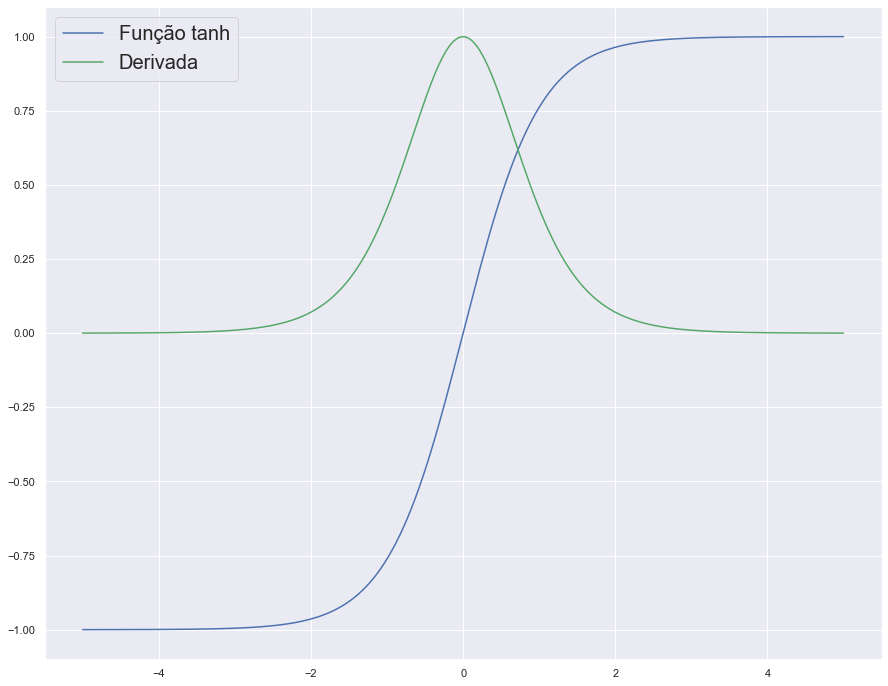
\includegraphics[width=12cm]{figuras/tanh}
\caption{Gráficos da função tangente hiperbólico e sua derivada.}
\label{fig:tanh}
\end{figure}

O próximo avanço é conseguido com a função de ativação linear retificada (\defi{RELU}). Essa função é quase a função identidade, exceto que na região negativa do domínio ela vale identicamente $0$. Ela não é derivável no ponto $x=0$, mas podemos estender a definição fixando seu valor em $1$ nesse ponto. Sua definição e de sua derivada estendida é dada por:

\[
ReLU(x)=max\{0, x\}   \quad \quad  ReLU'(x)=
	\begin{cases}
    	1, & \text{se } x\ge 0\\
    	0, & \text{c.c.}
	\end{cases}
\]

Podemos ver seus gráficos, na figura \ref{fig:relu}, a seguir. Usar essa função de ativação torna até mesmo a execução do código mais rápida, uma vez que não há cálculos matemáticos a serem feitos, apenas uma função de máximo que é trivial. Além disso, podemos notar que a derivada se mantém com o valor $1$ constante enquanto o neurônio é ativado, sendo uma forma de tentar resolver o problema do gradiente explodindo/desvanecendo, além de agilizar o processo de treinamento. 

\begin{figure}[htb]
\centering
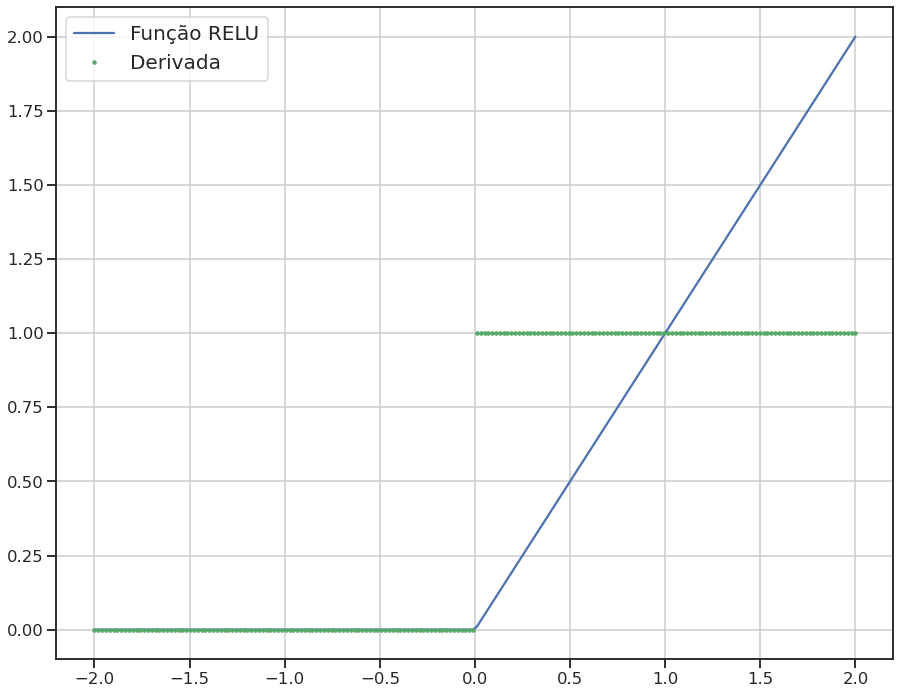
\includegraphics[width=12cm]{figuras/relu}
\caption{Gráficos da função \eng{RELU} e sua derivada.}
\label{fig:relu}
\end{figure}

Essa é a razão, conforme explica Facure \citep{matheus}, dessa função ter contribuido para o recente aumento de popularidade das redes neurais. Adicionalmente, Bing Xu \citep{xu_relu} ressalta que outra vantagem das funções do tipo \eng{RELU}, além de resolver o problema do gradiente explodindo/desvanescendo, é a de aumentar a velocidade da convergência do algoritmo de treinamento rumo a um mínimo da função de custos.

Uma desvantagem da função \eng{RELU} é a chance de neurônios serem desativados permanentemente, já que uma vez que ele zera, a função de ativação e sua derivada são ambos $0$, de forma que ele nunca mais irá aumentar durante o treinamento, tornando-se neurônios \emph{mortos}.

O próximo avanço foi dado pela função conhecida como \eng{Leaky RELU}. Quase identica à \eng{RELU}, exceto que na parte negativa do domínio ao invés de $0$ a função retorna $x/\alpha$, onde $\alpha \in (0, \infty)$. Isso já imediatamente corrige o problema dos neurônios desativados. A definição da função e de sua derivada, dada por Xu \citep{xu_relu}, é:

\[
LeakyReLU(x, \alpha) = 
\begin{cases}
    	x, & \text{se } x\ge 0\\
    	x/\alpha, & \text{c.c.}
	\end{cases}
\quad \quad  
LeakyReLU'(x, \alpha) =
	\begin{cases}
    	1, & \text{se } x\ge 0\\
    	\alpha, & \text{c.c.}
	\end{cases}
\]

A partir dos resultados dos estudos feitos por Xu \citep{xu_relu}, a função \eng{Leaky RELU}, e suas variações, se saíram consistentemente melhores do que a \eng{RELU} para as bases de dados de pequeno e médio portes. Além disso, ele testou a performance para diferentes valores de $\alpha$, obtendo os melhores resultados com $\alpha = 5.5$. Este parâmetro é conhecido como \defi{vazamento}, que dá o nome à função. Podemos ver o seu comportamento no gráfico da imagem \ref{fig:l_relu}.

\begin{figure}[htb]
\centering
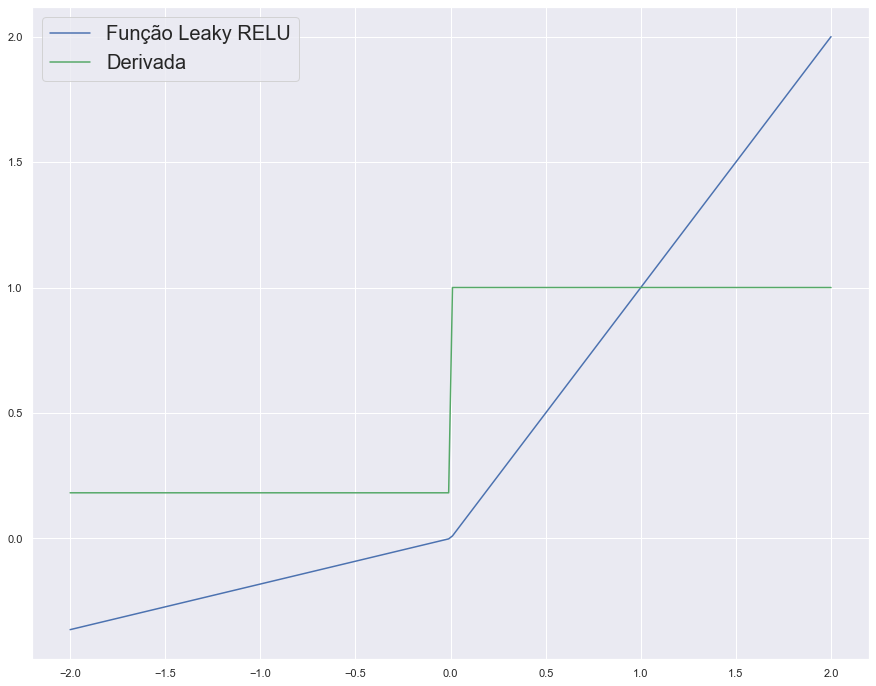
\includegraphics[width=12cm]{figuras/l_relu}
\caption{Gráficos da função \eng{Leaky RELU} e sua derivada.}
\label{fig:l_relu}
\end{figure}

Por fim, temos a função de unidade linear exponencial \eng{ELU}, proposta por Djork-Arné Clevert \citep{clevert}, que é definida, com $\alpha > 0$, por:

\[
ELU(x, \alpha)=
	\begin{cases}
    	x, & \text{se } x\ge 0\\
    	\alpha(e^x - 1), & \text{c.c.}
	\end{cases}
\quad \quad
ELU'(x, \alpha)=
	\begin{cases}
    	1, & \text{se } x\ge 0\\
    	ELU(x, \alpha)+\alpha, & \text{c.c.}
	\end{cases} 
\]

Em seu artigo, Clevert \citep{clevert} utiliza o valor $\alpha = 1$, e com a função \eng{ELU} conseguiu perfomances melhores, tanto de resultados mais corretos, quanto de velocidade de treinamento, em relação às funções \eng{RELU} e \eng{Leaky RELU} para as mesmas bases de dados avaliadas por XU \citep{xu_relu}, mesmo com o uso da função exponencial em sua definição o que em teoria deveria diminuir a performance do treinamento. Podemos observar o comportamento dessa função e de sua derivada, com $\alpha = 1$ no gráfico mostrado na figura \ref{fig:elu}.

\begin{figure}[htb]
\centering
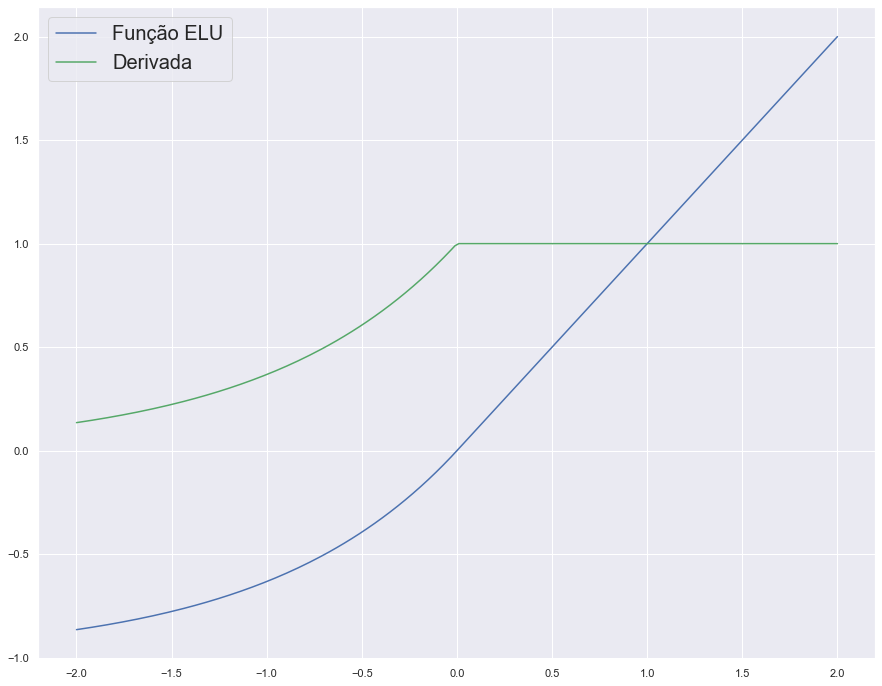
\includegraphics[width=12cm]{figuras/elu}
\caption{Gráficos da função \eng{ELU} e sua derivada.}
\label{fig:elu}
\end{figure}

Testes feitos em condições similares por Facure \citep{matheus}, mostram que essa diferença não é tão significativa em relação à \eng{Leaky RELU}, mas que ambas, \eng{Leaky RELU} e a \eng{ELU} são sim melhores do que a original \eng{RELU}, o que é consistente com o fato delas resolverem teoricamente as desvantagens dela. E são todas obviamente melhores escolhas do que a função \eng{sigmoid}, em todos os estudos acima citados.

Na prática, podemos testar qual função de ativação irá performar melhor para o problema que queremos resolver. A abordagem mais comum, conforme descrita por Facure \citep{matheus} é utilizar a função \eng{Leaky RELU} nas camadas ocultas, sendo o modo mais simples de obtermos bons resultados graças ao seu comportamento. Podemos avaliar a utilização das outras de acordo com o problema em questão, dado que algumas funções se saem melhor em alguns contextos específicos como é o caso da função \eng{sigmoid}.

\subsection{As camadas}

A classe \emph{Layer} representa uma camada de neurônios. Cada camada conecta-se com a sua camada anterior, com exceção da camada de entrada. Por essa razão, a rede perceptron possui um sentido único de conexão, que vai da entrada para a saída, passando por cada camada oculta. A classe é constituída de uma lista de objetos da classe \emph{Neuron}, uma referência à camada anterior e uma lista para armazenar as saídas dos seus neurônios.

O construtor de \emph{Layer} é responsável por inicializar seus neurônios. Nessa implementação todos os neurônios de uma camada irão usar a mesma função de ativação e a mesma taxa de aprendizagem. Além de receber esses parâmetros, o número de neurônios dessa camada, e a referência da camada anterior, o construtor inicializa os pesos de cada neurônio, lembrando que cada neurônio de uma camada possui a mesma quantidade de pesos do que a quantidade de neurônios da camada anterior, e também inicializa o viés de cada neurônio. 

Na listagem \ref{lst:layer_1} está o trecho do construtor que inicializa os pesos dos neurônios. Se a camada que estamos inicializando é a camada de entrada, então não criamos pesos e o viés, pois os valores de entrada serão utilizados diretamente como a saída dessa camada, este é o teste presente na linha 11 da listagem, pois a camada de entrada não possui referência a uma camada anterior já que ela é a primeira camada da rede.

A linha 12 de \ref{lst:layer_1} inicializa os pesos dos neurônios da camada. Para fazer isso utiliza uma função que está definida no script \texttt{util.py}, que sortea números aleatórios para esses pesos seguindo uma distribuição normal de média $0$ e desvio-padrão $0.3$ e além disso \emph{truncada} no intervalo $[-1, 1]$, para que nenhum peso esteja fora desse domínio e para que em média esse valor seja $0$. O viés é inicializado com um valor constante, próximo de zero, nesse caso com $0.01$.

\begin{scriptsize}
\estiloR
\begin{lstlisting}[caption={Trecho da classe \eng{Layer}}, label={lst:layer_1}, escapeinside={\%}]
class Layer:
    def __init__(self, previous_layer, num_neurons, learning_rate,
                 ativacao=None, der_ativacao=None):
        '''(Layer, int, float, Callable, Callable) -> None
        Construtor da Camada de Neurônios
        '''
        ...
        for i in range(num_neurons):
            pesos = None
            bias = None
            if previous_layer is not None:
                pesos = normal_t.rvs(len(previous_layer.neurons))
                bias = 0.01
            
            neuron = Neuron(pesos, bias, learning_rate, ativacao, der_ativacao)
            self.neurons = np.append(self.neurons, neuron)
\end{lstlisting}
\end{scriptsize}

Este procedimento é usado para tentar mitigar dois problemas que podem acontecer, conforme explicado por James Dellinger \citep{layers_1}. Se inicializarmos os pesos com muitos números não tão próximos de $0$, numa rede como muitos neurônios e muitas camadas, esses pesos podem somar-se rapidamente através das camadas, resultando em números com valores absolutos muito grandes na camada de saída o que pode prejudicar o treinamento e aprendizado da rede.

Se pelo contrário, inicializarmos todos os pesos com números muito próximos de $0$, ocorre o problema oposto, os neurônios tem seus valores zerados, tornando-se \emph{neurônios desativados}, que se tornam inúteis para o aprendizado já que serão ignorados durante o restante do treinamento. 

Dellinger \citep{layers_1} distute esses problemas no contexto de redes bem grandes, com mais de $100$ camadas, e exibe sua solução heurística que é utilizar uma distribuição normal (não-truncada) com média $0$ e com desvio-padrão $\sqrt{2/n}$, sendo $n$ o número de neurônios da camada anterior.

Para nossos fins didáticos, testei alguns desvios-padrão como $1$, $0.3$ e $0.1$, em um dos exemplos que serão mostrados ainda nesse capítulo, e dentre eles, o valor $0.3$ se saiu melhor sendo o suficiente para não explodir e nem desativar os neurônios da única camada oculta que foi usada na aplicação-exemplo em questão.

O desvio-padrão de $0.3$ auxilia na tarefa de restringir os valores no intervalo $[-1, 1]$, sem que precisemos truncar muitos valores o que poderia aumentar a massa de probabilidade dos extremos $-1$ e $1$, já que valores mais distantes da média do que $3$ vezes o desvio-padrão são raramentes obtidos de uma distribuição normal. 

Após inicializar cada neurônio, salvamos ele na lista de neurônios dessa camada, que é um dos atributos de classe discutidos no primeiro parágrafo. A próxima tarefa de uma camada é processar as entradas recebidas e retornar as saídas. Podemos observar esse comportamento na listagem \ref{lst:layer_2}.

\newpage

\begin{scriptsize}
\estiloR
\begin{lstlisting}[caption={Trecho da classe \eng{Layer}}, label={lst:layer_2}, escapeinside={\%}]
def outputs(self, inputs):
        '''(list[float]) -> list[float]
        Armazena em cache as saidas dos neuronios e a retornam
        Se for uma camada de entrada, usa elas diretamente
        '''
        if self.previous_layer is None:
            self.output_cache = inputs
        else:
            self.output_cache = np.array([n.output(inputs) for n in self.neurons])
        return self.output_cache
\end{lstlisting}
\end{scriptsize}

A camada de entrada não processa os dados, usando-os diretamente. As demais camadas devem processar cada neurônio, usando seu próprio método de processamento, aplicando a transformação linear e em seguida a função de ativação. O resultado é armazenado numa lista \eng{numpy} que é o atributo de classe \texttt{output$\_$cache}, que armazena as saídas dessa camada para uso posterior; por fim, a lista das saídas da camada é retornada.

A última tarefa da classe \eng{Layer} é calcular os termos $\Delta$ definidos pelas equações \ref{retro:15} e \ref{retro:16}, que definem respectivamente o cálculo que é feito se estamos calculando as derivadas para as camadas ocultas e o cálculo feito para a camada de saída. As duas versões são exibidas na listagem \ref{lst:layer_3} abaixo.

\begin{scriptsize}
\estiloR
\begin{lstlisting}[caption={Trecho da classe \eng{Layer}}, label={lst:layer_3}, escapeinside={\%}]
def calcular_delta_camada_de_saida(self, expected):
        '''(list[float]) -> None'''
        for i, neuron in np.ndenumerate(self.neurons):
            der_cost = expected[i[0]] - self.output_cache[i]
            neuron.delta = neuron.der_ativacao(neuron.output_cache) * der_cost

    def calcular_delta_camada_oculta(self, next_layer):
        '''(Layer) -> None'''
        for i, neuron in np.ndenumerate(self.neurons):
            next_weights = np.array([n.weights[i[0]] for n in next_layer.neurons])
            next_deltas = np.array([n.delta for n in next_layer.neurons])
            der_cost = np.dot(next_weights, next_deltas)
            neuron.delta = neuron.der_ativacao(neuron.output_cache) * der_cost
\end{lstlisting}
\end{scriptsize}

Os algoritmos são as traduções quase literais das equações \ref{retro:15} e \ref{retro:16}. Podemos ver a natureza recursiva da regra da cadeia nas 2 linhas finais, onde usamos os deltas calculados da próxima camada para calcular os deltas da camada atual. O caso base é a função que calcula o delta da camada de saída. A lógica que orquestra essa recursão está implementada na próxima classe.

\subsection{A rede}

A classe \eng{Network} representa a rede neural como um todo. Ela armazena uma lista de camadas, ou seja, objetos do tipo \eng{Layer}, a partir dos parâmetros que recebe em seu construtor, que são a estrutura da rede que será criada, que é um vetor de inteiros que representam as quantidades de neurônios para cada camada. Além disso, recebe a taxa de aprendizado que será utilizada em toda a rede, nessa versão, e quais as funções de ativação que serão utilizadas nas camadas ocultas e na camada de saída.

A listagem \ref{lst:network_1} exibe o trecho do construtor que cria cada camada e insere na lista de camadas do objeto da classe atual. A camada de entrada não possui camada anterior, nem função de ativação. Além disso, a camada de saída pode utilizar uma função de ativação diferente daquela utilizada pelas camadas ocultas, que usarão a mesma.

\begin{scriptsize}
\estiloR
\begin{lstlisting}[caption={Trecho da classe \eng{Network}}, label={lst:network_1}, escapeinside={\%}]
class Network:
    def __init__(self, layer_structure, taxa, ativacoes):
        '''(list[int], float, Tuple[Callable]) -> None'''
        ...
        self.layers = np.array([], dtype=np.float64)
        self.estrutura = layer_structure

        # camada de entrada
        input_layer = Layer(None, self.estrutura[0], taxa)
        self.layers = np.append(self.layers, input_layer)

        # camadas oculta(s)
        for previous, qtd_neurons in np.ndenumerate(self.estrutura[1::l]):
            next_layer = Layer(self.layers[previous[0]], qtd_neurons, taxa,
                               ativacoes[0], ativacoes[1])
            self.layers = np.append(self.layers, next_layer)

        # camada de saída
        output_layer = Layer(self.layers[-1], self.estrutura[-1], taxa,
                               ativacoes[2], ativacoes[3])
        self.layers = np.append(self.layers, output_layer)
\end{lstlisting}
\end{scriptsize}

A primeira tarefa da classe Network é o de processar entradas, fazendo elas atravessarem a rede, camada a camada, até a camada de saída, e retornar as saídas obtidas. É o processo de \eng{feedforward} explicado no início do capítulo. Sua implementação mesmo para o caso geral de multi-camadas é bem simples, conforme exibido na listagem \ref{lst:network_2} abaixo.

\begin{scriptsize}
\estiloR
\begin{lstlisting}[caption={Trecho da classe \eng{Network}}, label={lst:network_2}, escapeinside={\%}]
def feedforward(self, entrada):
    '''(list[float]) -> list[float]'''
    ...
    saida = self.layers[0].outputs(entrada)
    for i in range(1, len(self.layers)):
        saida = self.layers[i].outputs(saida)
    return saida
\end{lstlisting}
\end{scriptsize}

A próxima tarefa é treinar a rede, passando uma lista de entradas e saídas esperadas, realizando o procedimento de \eng{backpropagate} para atualizar os pesos e viéses dos neurônios de cada camada, tudo isso em sequência, para cada entrada fornecida. É o que está literalmente implementado na listagem \ref{lst:network_3} abaixo.

\begin{scriptsize}
\estiloR
\begin{lstlisting}[caption={Trecho da classe \eng{Network}}, label={lst:network_3}, escapeinside={\%}]
def train(self, entradas, saidas_reais):
    '''(list[list[floats]], list[list[floats]]) -> None'''
    ...
    for i, xs in enumerate(entradas):
        ys = saidas_reais[i]
        _ = self.feedforward(xs)
        self.backpropagate(ys)
        self.update_weights()
        self.update_bias()
	return saida
\end{lstlisting}
\end{scriptsize}

Cada chamada à função \eng{train} significa o procedimento de treinamento sendo executado uma única vez. Cada vez que a rede é treinada dizemos que ela avançou em uma \defi{época} de treinamento. O treinamento consiste em primeiramente executar o \eng{feedforward} para uma entrada, para que as camadas possam armazenar as saídas correspondentes aos valores atuais de seus parâmetros, os pesos e viéses, assim como as saídas em seus atributos \eng{output$\_$cache}, que serão usados pelo método \eng{backpropagate} a seguir, de acordo com as equações que derivamos para o processo de treinamento.

O funcionamento do método \eng{backpropagate} pode ser visto na listagem \ref{lst:network_4} a seguir. Tudo o que ele faz aqui é calcular os deltas das camadas, na ordem correta, começando pela camada de saída, e depois percorrendo as demais camadas do final para o início da rede, fazendo a chamada para cada objeto da classe \eng{Layer} que constitui a rede.

\begin{scriptsize}
\estiloR
\begin{lstlisting}[caption={Trecho da classe \eng{Network}}, label={lst:network_4}, escapeinside={\%}]
def backpropagate(self, saidas_reais):
    '''(list[float]) -> None
    Calcula as mudanças em cada neurônio com base nos erros da saída
    em comparação com a saída esperada
    '''
    # calcula delta para os neurônios da camada de saída
    last_layer = len(self.layers) - 1
    self.layers[last_layer].calcular_delta_camada_de_saida(saidas_reais)
    
    # calcula delta para as camadas ocultas, da saída para o início da rede
    for l in range(last_layer - 1, 0, -1):
        self.layers[l].calcular_delta_camada_oculta(self.layers[l + 1])
\end{lstlisting}
\end{scriptsize}

A seguir, atualiza-se os pesos e os viéses com os métodos correspondentes, que podem ser visualizados na listagem \ref{lst:network_5}. Como os valores são todos armazenados nos atributos de estado dos neurônios e das camadas, implementamos diretamente as contas das equações que obtemos para o método do gradiente e da regra da cadeia da retroprogação. Dessa forma, o que fazemos na classe \eng{Network} é basicamente traduzir a matemática para a sintaxe da linguagem Python.

\newpage

\begin{scriptsize}
\estiloR
\begin{lstlisting}[caption={Trecho da classe \eng{Network}}, label={lst:network_5}, escapeinside={\%}]
def update_weights(self):
    '''(None) -> None'''
    ...
    for layer in self.layers[1:]: # pula a camada de entrada
        for neuron in layer.neurons:
            for w in range(len(neuron.weights)):
                neuron.weights[w,] = neuron.weights[w,] + (neuron.learning_rate
                     * (layer.previous_layer.output_cache[w]) * neuron.delta)

def update_bias(self):
    '''(None) -> None'''
    ...
    for layer in self.layers[1:]: # pula a camada de entrada
        for neuron in layer.neurons:
            neuron.bias = neuron.bias + neuron.learning_rate * neuron.delta
\end{lstlisting}
\end{scriptsize}

A próxima responsabilidade da classe \eng{Network}, uma vez que já foi treinada, é fazer a previsão de classes de novos dados de entrada. Isto é feito pelo método mostrado na listagem \ref{lst:network_6}. Isto significa simplesmente processar as entradas fornecidas pelo método \eng{feedforward}, que usará os parâmetros que foram ajustados anteriormente para fazer os cálculos. 

\begin{scriptsize}
\estiloR
\begin{lstlisting}[caption={Trecho da classe \eng{Network}}, label={lst:network_6}, escapeinside={\%}]
def predict(self, entradas, interpretar):
    '''(list[list[floats]], Callable) -> list[list[floats]]
    '''
    self.previsoes = np.array([], dtype=np.float64)
    for entrada in entradas:
        self.previsoes = np.append(self.previsoes, interpretar(self.feedforward(entrada)))
    return self.previsoes.reshape(-1, 1)
\end{lstlisting}
\end{scriptsize}

Ao final, os dados da última camada são uma lista, isto é, um vetor de valores reais, que são interpretados por uma função que é passada por parâmetro que identifica a qual classe, previamente definida, pertence esse vetor de saída. A lógica dessa interpretação é externa à classe \eng{Network} e será vista mais adiante. A lista de classes preditas em formato \eng{numpy} é retornada.

A última responsabilidade dessa classe é calcular uma métrica de avaliação para esta rede, que irá servir de avaliação do quão boa a rede é para classificar os dados utilizados. A métrica mais simples a ser utilizada é a \defi{acurácia} da previsão. Ela basicamente mede a proporção de classificações corretas dentre todas as classificações realizadas para um conjunto de dados. Essa lógica bem simples é implementada na listagem \ref{lst:network_7} abaixo. 

\begin{scriptsize}
\estiloR
\begin{lstlisting}[caption={Trecho da classe \eng{Network}}, label={lst:network_7}, escapeinside={\%}]
def validate(self, esperados):
    '''(list[list[floats]], list[list[floats]], Callable) -> float
    '''
    ...
    corretos = 0
    for y_pred, esperado in zip(self.previsoes, esperados):
        if y_pred == esperado:
            corretos += 1
    acuracia = corretos / len(self.previsoes)
    return acuracia
\end{lstlisting}
\end{scriptsize}

Nota-se que ela utiliza as previsões salvas no atributo de classe que é atualizado toda vez que executamos o método \eng{predict}, acima. As classes esperadas são passadas como parâmetro, uma vez que estamos lidando no \eng{Perceptron} com uma aprendizagem supervisionada. Dessa forma, ao treinarmos a rede utilizamos um conjunto de dados para os quais já sabemos as classes, e ainda dividimos esse conjunto em duas partes, as quais chamamos de \defi{conjunto de treino} e de \defi{conjunto de teste ou validação}.

Treinamos a rede com o conjunto de treino, que deve sempre ser a maior parte de nossa partição, uma vez que é a partir dele que iremos usar o \eng{backpropagate} para aproximar as saídas da rede às saídas esperadas contidas no conjunto. Géron \citep{hands} cita que tipicamente escolhemos aleatoriamente $20\%$ dos dados como nosso conjunto de teste, ficando o restante como o conjunto de treino. A seguir, podemos calcular a acurácia da classificação do conjunto de treino, e a seguir prever e medir a acurácia do conjunto de teste para comparar os resultados. 

Naturalmente a acurácia para o conjunto de teste tende a ser menor, mas não pode ser muito menor, senão dizemos que nossa rede sofre de um problema de classificação conhecido como \defi{overfitting}, ou sobreajuste, o que significa que ela está boa para lidar com o conjunto com o qual foi treinado, o que era esperado dado que foi construída para isso, mas sofre para classificar dados novos, com os quais não foi treinada, e não é isso o que queremos. 

O que queremos é justamente o contrário, que nossa rede, ou seja, nosso algoritmo de aprendizagem seja bom em \defi{generalizar} os dados de entrada que fornecemos a ele. Anas Al-Masri \citep{network_1} define o termo generalização como a habilidade do modelo para fornecer saídas sensíveis para conjuntos de entradas que ele nunca viu antes. 

Dentre as várias técnicas existentes para melhorar a generalização/prevenir o \eng{overfitting} estão a inicialização dos pesos dos neurônios segundo uma distribuição normal de média zero, procedimento explicado anteriormente. Outra técnica é denominada de \defi{dropout}, a qual Amar Budhiraja \citep{network_2} define como ignorar alguns neurônios, escolhidos aleatoriamente, durante o treinamento da rede, isto é, não calculamos deltas durante uma execução do \eng{backpropagate} e nem usamos seu valor em consideração quando processamos uma entrada na rede como o \eng{feedforward}.

É como se deliberadamente ``desativássemos'' alguns neurônios durante a fase de treinamento, de forma a diminuir o sobreajuste aos dados de treino, uma vez que, segundo Budhiraja \citep{network_2} esse procedimento previne que todos os neurônios se tornem dependentes um dos outros, isto é, que a derivada (da função de custo) de cada um se torne dependente das derivadas de todos os outros, criando uma mútua dependência geral para a diminuição do erro, diminuindo assim o poder individual que cada um teria se fossem ajustados de forma mais independente em função de sua contribuição para o custo total da rede.

Em nosso \eng{Perceptron} didático optei por não implementar o procedimento de \eng{dropout}, já que o objetivo dessa versão aqui demonstrada não é fornecer um modelo que seja utilizado em problemas reais, mas apenas didáticos. Em contrapartida essa técnica está presente e pode ser utilizada nas bibliotecas de redes neurais que usaremos na parte prática do trabalho.

\subsection{A classe \eng{Perceptron}}

A última classe implementada, não foi baseada em um exemplo, mas criada a partir da necessidade de encapsular o comportamento da rede, para facilitar os testes do seu funcionamento que iremos realizar. Já discutimos sobre as diferentes taxas de aprendizagem para o gradiente descendente, discutimos sobre as diferentes funções de ativação que podem ser utilizadas nas redes neurais, assim como a sua topologia no que se refere apenas à quantidade de neurônios e a quantidade de camadas de neurônios.

Esses são basicamente os atributos que teremos que ajustar de acordo com a necessidade que os dados utilizados em nosso aprendizado irão criar. Dessa forma criamos a classe \eng{Perceptron} que possui um construtor que irá lidar com a seleção dessas opções. Na listagem \ref{lst:percep_1} está apenas a definição de seu construtor e a documentação explicativa.

\begin{scriptsize}
\estiloR
\begin{lstlisting}[caption={Trecho da classe \eng{Perceptron}}, label={lst:percep_1}, escapeinside={\%}]
class Perceptron():
    def __init__(self, N=[1], M=50, ativacao="l_relu", taxa=0.001, debug=0):
	    '''(None, str, list[int], int, float, float, str, float) -> None
	    Construtor da minha classe Perceptron
	    Parâmetros da classe:
	        *N: quantidade de neurônios da camada oculta, podendo ser
	            especificada um vetor de várias camadas ocultas ou apenas
	            uma.
	        *M: quantidade de treinamentos desejada, denominado de número
	            de "épocas" da rede, o valor padrão é 50;
	        *ativacao: escolha de uma das funções de ativação disponíveis
	            para a(s) camada(s) oculta(s).
	        *taxa: taxa de aprendizagem, padrão de 0.001
	        *debug: flag para exibição de parâmetros durante o treinamento
	    '''
	    ...
\end{lstlisting}
\end{scriptsize}

No construtor é feita uma seleção dentre as funções de ativação existentes no script \eng{util.py}, de forma que só precisamos passar um texto com o nome da função, que o construtor irá selecionar a função e sua derivada para posteriormente informá-las à classe \eng{Network}. Deixamos por padrão a escolha da função de ativação \eng{Leaky RELU}, de acordo com a orientação geral dada por Facure \citep{matheus}.

O parâmetro $M$ define a quantidade inicial padrão de \defi{épocas} que serão treinadas. Uma época corresponde a uma passagem do conjunto de treino pelo \eng{feedforward} e a seguir pelo \eng{backpropagation}, ou seja, configura um único ajuste dos parâmetros através de nosso algoritmo de treinamento.

A arquitetura de camadas padrão definida pelo parâmetro $N$ não tem de fato esse papel, serve apenas para uma validação existente no construtor para que não permita a passagem de uma quantidade $\leq 0$ de camadas ou de neurônios. Se quiséssemos uma arquitetura de $3$ camadas com $4, 5, $ e $6$ neurônios cada, por exemplo, então o parâmetro passado durante a criação de um objeto \eng{Perceptron} deveria ser $N = [4, 5, 6]$.

Outra tarefa do construtor é criar um objeto da classe \eng{OneHotEncoder}\footnote{\url{https://scikit-learn.org/stable/modules/generated/sklearn.preprocessing.OneHotEncoder.html}} da biblioteca \eng{scikit-learn}\footnote{\url{https://scikit-learn.org/stable/index.html}}. Essa é uma das mais famosas e mais utilizadas bibliotecas da linguagem Python para tarefas de aprendizado de máquina. É a biblioteca utilizada pela maioria dos autores dos livros-textos da área de ciência de dados, como por exemplo Géron \citep{hands} e Grus \citep{data}.

Esse objeto codificador (\eng{encoder}) é salvo como um atributo de classe: \texttt{self.\_enc}, e será utilizado no método de treinamento para criar automaticamente as classes numéricas a partir das classes fornecidas pelos conjuntos de treinamento e validação. Essas classes numéricas representam cada classe no formato de um vetor com todos os componentes zerados exceto um, o que identifica unicamente as classes.

Suponha, por exemplo, que estamos treinando um conjunto de fotos que possuem as classes \emph{cachorro}, \emph{gato} e \emph{rato}. A função codificadora poderá transformar a palavra \emph{cachorro} no vetor $[1, 0, 0]$, \emph{gato} no vetor $[0, 1, 0]$ e \emph{rato} no vetor $[0, 0, 1]$. De forma que estes serão os valores esperados para os $3$ neurônios de saída que nossa rede obrigatoriamente deverá ter (número de classes = número de neurônios de saída). A ordem dessa codificação é irrelevante, sendo gerenciada internamente pela classe \eng{OneHotEncoder}.

A seguir, no método utilizado para treinar a rede, que recebe os dados de entrada e as classes esperadas correspondentes a cada entrada, o primeiro passo é fazer essa codificação. O primeiro trecho do método \texttt{treinar} está na listagem \ref{lst:percep_2}.

\begin{scriptsize}
\estiloR
\begin{lstlisting}[caption={Trecho da classe \eng{Perceptron}}, label={lst:percep_2}, escapeinside={\%}]
def treinar(self, x_train, y_train, M=0):
    '''(np.array, np.array, int) -> None
    Processo de treinamento da rede neural
    1- Tratar os dados, obtendo as classes das respostas
    2- Treinar um número M de épocas
    3- Armazenar no objeto o estado final da rede, 
    com os pesos e vieses ajustados pelo treinamento
    '''
    # onehotencoder extrai as classes únicas já ordenadas alfabeticamente
    y_encoded = self._enc.fit_transform(y_train)
    classes = self._enc.categories_[0]
\end{lstlisting}
\end{scriptsize}

Nessa classe e nos exemplos subsequentes neste trabalho, sempre nomeio o conjunto dos dados de treino de \texttt{x\_train} e \texttt{y\_train}, e do conjunto de teste de \texttt{x\_test} e \texttt{y\_test}. A letra $x$ indica que é o conjunto de dados de entrada e $y$ indica as classes esperadas de classificação. No trecho acima usamos a classe \eng{OneHotEncoder} para transformar quaisquer formatos que as classes forem informadas nos vetores numéricos que serão os valores esperados da saída da rede.

O próximo trecho de código irá se encarregar de criar a estrutura geral da rede, ao final criando um objeto da classe \eng{Network} e salvando-o como um atributo de classe. É o que está presente na listagem \ref{lst:percep_3}. Os dados de entrada são esperados no formato de lista do tipo \eng{numpy}, dessa forma a primeira linha do trecho obtém a quantidade de características (\eng{features}) dos dados de entrada, ou seja, das variáveis explicativas do modelo, através do método \texttt{shape(1)} do tipo \eng{numpy}, essa será a quantidade de neurônios da camada de entrada da rede, um para cada característica.

Usando o exemplo das fotos de animais, os pixels da foto seriam as variáveis explicativas para um modelo de classificação, assumindo que todas as fotos possuem a mesma quantidade de pixels e que cada pixel possui apenas um valor de intensidade de cinza, ou outra cor única qualquer. Se utilizássemos fotos coloridas, com por exemplo, as intensidades de $3$ cores diferentes por pixel, então o número de variáveis explicativas de nosso modelo seria $3n$, sendo $n$ o número de pixels da foto.

\begin{scriptsize}
\estiloR
\begin{lstlisting}[caption={Trecho da classe \eng{Perceptron}}, label={lst:percep_3}, escapeinside={\%}]
	neurons_in = x_train.shape[1]

	if self.network is None:
	    neurons_out = len(self.classes)
	    for i in range(len(self.N)):
	        if len(self.N) == 1 and self.N[0] < neurons_out:
	            self.N[0] = min(int(np.ceil(neurons_in*2/3 + neurons_out)), neurons_in)
	    
	    rede = []
	    rede.append(neurons_in)
	    for hidden in self.N:
	        rede.append(hidden)
	    rede.append(neurons_out)
	    
	    ativacoes = (self.ativacao, self.der_ativacao, 
	                 self.ativacao_saida, self.der_ativacao_saida)

	    self.network = Network(np.array(rede), self.taxa, ativacoes)
\end{lstlisting}
\end{scriptsize}

A seguir, o método irá criar a estrutura da rede, se essa é a primeira vez que o objeto estiver sendo utilizado para o treinamento, do contrário ele irá realizar outras $M$ épocas de treinamento, a partir dos dados existentes na rede. 

Obtém-se a quantidade de neurônios para a camada de saída a partir da quantidade de classes identificadas. A seguir ele utiliza as quantidades de neurônios para as camadas ocultas se estas foram previamente informadas manualmente durante a criação da classe, ou então, é feito um cálculo, para que seja utilizada uma quantidade apropriada de neurônios para a primeira camada oculta, que pode ser a única camada oculta por padrão.

Essa quantidade apropriada é definida por Jeff Heaton \citep{layers_2} como sendo $2/3$ da quantidade de neurônios de entrada mais a quantidade de neurônios de saída. Esta é uma das `regras de ouro' que ele descobriu empiricamente pois se mostraram as regras mais gerais para garantir o bom funcionamento da rede em vários casos. Outra regrinha que ele encontrou, que é mais geral mas que incluí esta é que a quantidade de neurônios de uma camada oculta única deve ser tal que seja menor que a quantidade de neurônios de entrada mas maior que a quantidade de neurônios de saída.

Naturalmente o treinamento aceita quaisquer número de camadas ocultas e de neurônios em cada camada, apenas não há garantias de que o treinamento irá suceder sem ocorrer o problema do gradiente explodindo/desaparecendo. Mesmo a utilização das regrinhas de Heaton \citep{layers_2} não asseguram esse sucesso do treinamento, apenas testes com outras quantidades de neurônios e camadas, e com outras funções de ativação e taxas de aprendizado que poderão resultar eventualmente num treinamento bem sucedido, caso essas opções-padrão não sejam suficientes.

Essa é uma dificuldade inerente das redes neurais, ainda mais quando tenta lidar com conjuntos de dados muito grandes e com um grande número de variáveis explicativas. Essa é uma das razões principais para ser preferível a utilização de uma biblioteca já consolidade e com muitos anos de desenvolvimento e ajustes por muitos desenvolvedores e cientistas de dados ao redor do mundo.

O próximo trecho, na listagem \ref{lst:percep_4} é o trecho principal deste método, é o treinamento \eng{backpropagate} feito um número $M$ de épocas. São passados como parâmetros os dados de entrada, e as classes esperadas já codificadas. Ao final desse treinamento, a rede está salva no atributo de classe \texttt{self.network} com os parâmetros já ajustados e prontos para serem utilizados para validação e previsão de novos dados.

\begin{scriptsize}
\estiloR
\begin{lstlisting}[caption={Trecho da classe \eng{Perceptron}}, label={lst:percep_4}, escapeinside={\%}]
    for _ in self.tqdm(range(self.M)):
        self.network.train(x_train, y_encoded)
\end{lstlisting}
\end{scriptsize}

O próximo método realiza a previsão das classes a partir dos dados informados, simplesmente utilizando a função da classe \eng{Network} criada para isso. É o que está na listagem \ref{lst:percep_5}, abaixo. 

\begin{scriptsize}
\estiloR
\begin{lstlisting}[caption={Trecho da classe \eng{Perceptron}}, label={lst:percep_5}, escapeinside={\%}]
def prever(self, X, interpretar=None):
    '''(np.array, Callable) -> np.array'''
    ...
    if interpretar is None:
        return self.network.predict(X, self.reinterpretar_saidas)
    return self.network.predict(X, interpretar)
\end{lstlisting}
\end{scriptsize}

Por padrão a função que irá interpretar os neurônios de saída, convertendo-os em uma classe, foi criada da forma como será mostrada na listagem \ref{lst:percep_6}, a seguir.

\begin{scriptsize}
\estiloR
\begin{lstlisting}[caption={Trecho da classe \eng{Perceptron}}, label={lst:percep_6}, escapeinside={\%}]
def reinterpretar_saidas(self, saidas):
    '''(array) -> np.array
    '''
    maximo = max(saidas)
    saida = np.array([int(x == maximo) for x in saidas])
    return self._enc.inverse_transform(saida.reshape(1, -1))
\end{lstlisting}
\end{scriptsize}

Essa função realiza a interpretação padrão dos neurônios de saída, primeiramente eles são convertidos em vetores com identificação única, ou seja, no formato $[0, \ldots,0, 1, 0, \ldots, 0]$, sendo que a posição que irá receber $1$ é aquela que tiver originalmente o valor máximo, ou seja, mais distante de $0$, e o restante será convertido em zeros. Dessa forma, basta utilizarmos a decodificação inversa do objeto \eng{OneHotEncoder}, que está salvo no atributo de classe, e daí obtemos qual a classe mais provável à qual pertence o dado de entrada que foi processado pela rede.

Isto nos mostra que uma possível interpretação dos neurônios de saída é que cada um possui uma probabilidade de que o dado pertença àquela classe indexada na mesma posição a qual esse neurônio está na camada de saída. Se usarmos como exemplo nosso modelo fictício dos animais, ao processar uma foto, a rede iria devolver os valores dos neurônios de saída, por exemplo, como o seguinte vetor: $[0.002, 0.976, 0.013]$. Pode-se dizer que há uma probabilidade maior de que essa foto pertença à segunda classe, que digamos ser a classe \emph{Gatos}, por exemplo.

O que a função \texttt{reinterpretar\_saidas} faz é converter esse vetor de saídas da rede no vetor $[0, 1, 0]$, que agora está no formato das classes numéricas geradas por nosso objeto codificador. Dessa forma, executar uma decoficação com esse mesmo objeto, que havia originalmente codificado a palavra \emph{Gato} no vetor $[0, 1, 0]$, irá fazer a operação inversa, retornando a palavra \emph{Gato} como sendo a classe mais provável para a foto processada.

Alternativamente podemos utilizar outra função de interpretação dos dados de saída, devendo ser informada diretamente por referência para o método \texttt{prever}.

Por razões didáticas, ou mesmo em casos em que não queremos obter classes diretamente a partir dos neurônios de saída, mas queremos observar diretamente os valores calculados pela rede sem interpretação, criei um método que realiza apenas o \eng{feedforward} para uma lista de entradas fornecidas como parâmetro. É o que vemos na listagem \ref{lst:percep_7}, a seguir.

\begin{scriptsize}
\estiloR
\begin{lstlisting}[caption={Trecho da classe \eng{Perceptron}}, label={lst:percep_7}, escapeinside={\%}]
def processar(self, X):
    '''(np.array) -> np.array'''
    ...
    saidas = []
    for x in X:
        saidas.append(self.network.feedforward(x))
    return np.array(saidas)
\end{lstlisting}
\end{scriptsize}

Por fim, podemos querer observar qual o erro, ou custo, que nossa rede está produzindo para um dado par de conjuntos de entrada e saídas esperadas. Para isso criei o método \texttt{funcao\_erro} exibido na listagem \ref{lst:percep_8}, a seguir. 

\begin{scriptsize}
\estiloR
\begin{lstlisting}[caption={Trecho da classe \eng{Perceptron}}, label={lst:percep_8}, escapeinside={\%}]
def funcao_erro(self, X, Y):
    '''(np.array, np.array) -> float'''
    ...
    y_encoded = self._enc.fit_transform(Y)
    return self.network.mse(X, y_encoded)
\end{lstlisting}
\end{scriptsize}

Ele utiliza a função de erro que está implementada na classe \eng{Network}, que é a função de custo que utilizamos como base para a criação de nosso algoritmo de otimização, o erro quadrático médio (MSE), também conhecido como a norma euclidiana do vetor distância entre os vetores das saídas esperadas e o das saídas obtidas pela rede.

Em todos os trechos da classe \eng{Perceptron} acima, várias linhas estão ocultas sob o símbolo de reticências, são linhas que fazem verificações dos dados utilizados e do estado atual do objeto, se ele pode ser usado para previsão por exemplo, ou seja, se já foi treinado previamente, entre outras verificações gerais para um bom funcionamento.

\section{Exemplo de utilização do \eng{perceptron}}

Para demonstrar a utilização da versão aqui implementada da rede \eng{perceptron}, resolvi utilizar aquela que é considerada a base de dados de entrada no mundo da ciência de dados, a base MNIST (\eng{Modified National Institute of Standards and Technology}) de números escritos à mão compilada originalmente pela Universidade de Nova York\footnote{Disponível originalmente em \url{http://yann.lecun.com/exdb/mnist/}.}.

A versão oficial da base de dados consistem em $60$ mil imagens de dimensões $28 \times 28$ pixels. Cada imagem é uma foto de um dígito manuscrito entre $0$ e $9$, sendo que a proporção de cada dígito é aproximadamente de um décimo, além disso a base contém a informação dos valores nominais de cada número, o que torna essa base de dados muito útil para validar modelos de aprendizado supervisionado, antes que sejam utilizados em casos reais. Exemplos de fotos estão na figura \ref{fig:mnist_fig}.

\begin{figure}[htb]
\centering
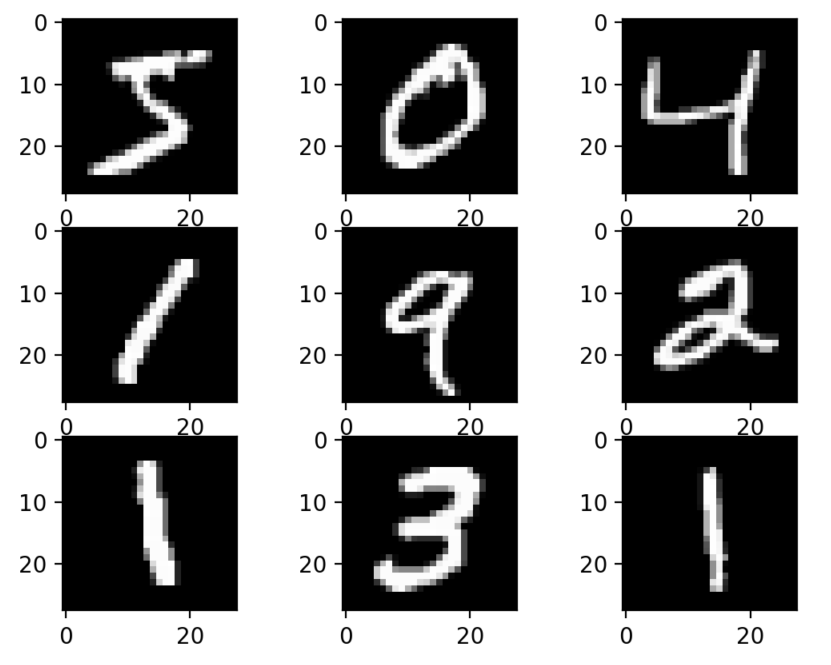
\includegraphics[width=8cm]{figuras/mnist}
\caption{Exemplos de fotos da base de dados MNIST de números manuscritos.\footnote{Extraído de \url{https://3qeqpr26caki16dnhd19sv6by6v-wpengine.netdna-ssl.com/wp-content/uploads/2019/02/Plot-of-a-Subset-of-Images-from-the-MNIST-Dataset-1024x768.png}}}
\label{fig:mnist_fig}
\end{figure}

É exatamente esse o objetivo aqui, testar nossa implementação didática do \eng{perceptron}. Para isso, o primeiro passo foi obter uma versão mais \emph{leve} da base de dados, com as fotos redimensionadas para $8 \times 8$ pixels, o que implica em $64$ variáveis explicativas e mesmo número de neurônios de entrada. Além disso essa base possui apenas $1.800$ fotos etiquetadas. A base original de $28^2 = 784$ pixels já se mostrou grande demais para essa implementação conseguir lidar em tempo hábil.\footnote{Em tentativas que fiz com a base original, meu computador ficou calculando deltas por quase 2 horas sem completar uma só época de treinamento.}

A base foi importada através da biblioteca \eng{sklearn}, que já possui opções para fazer download automático para o programa em execução de várias versões da base MNIST. O código da listagem \ref{lst:mnist_1} mostra a importação e também o próximo passo, que é separar a base nos conjuntos de treino, com $85\%$ dos dados, e de validação com os $15\%$ restantes.

\begin{scriptsize}
\estiloR
\begin{lstlisting}[caption={Trecho do script \eng{mnist\_test.py}}, label={lst:mnist_1}, escapeinside={\%}]
# obtendo o conjunto de imagens de numeros escritos
from sklearn.datasets import load_digits
mnist = load_digits()

# dividindo a base nos conjuntos de treino e de teste
N = int(mnist.data.shape[0]*0.85)
x_train, y_train = mnist.data[:N], mnist.target[:N].astype(np.uint8)
x_test, y_test = mnist.data[N:], mnist.target[N:].astype(np.uint8)
\end{lstlisting}
\end{scriptsize}

A implementação está tão fácil de utilizar, que para a tarefa de treinar a classificação dos números digitados, não precisamos de mais de meia dúzia de linhas de código, mostradas na listagem \ref{lst:mnist_2}.

\begin{scriptsize}
\estiloR
\begin{lstlisting}[caption={Trecho do script \eng{mnist\_test.py}}, label={lst:mnist_2}, escapeinside={\%}]
perceptron = Perceptron(taxa=0.001, ativacao="l_relu", N=[48, 24])
perceptron.treinar(x_train, y_train, M=25)

y_train_pred = perceptron.prever(x_train)
y_test_pred = perceptron.prever(x_test)

score = Scores(y_test, y_test_pred)
score.exibir_grafico()
\end{lstlisting}
\end{scriptsize}

Basicamente, uma rede é criada com a estrutura de uma camada de entrada com $64$ neurônios, quantidade obtida automaticamente pela classe a partir das dimensões da lista de dados informada (\eng{y\_train}), duas camadas ocultas com $48$ e $24$ neurônios cada, com taxa de aprendizado $0.001$ e a função de ativação \eng{Leaky RELU}, ambos ajustados empiricamente sendo o que se saíram melhores em acurácia. A segunda linha realiza o treinamento com $25$ épocas, informando a lista de imagens e a lista das classificações conhecidas.

As duas últimas linhas dessa listagem fazem a comparação dos valores previstos com os valores já conhecidos da classificação, para conhecermos a acurácia de nosso modelo de aprendizado. Abaixo nas figuras \ref{fig:mnist_treino} e \ref{fig:mnist_test} está uma exibição gráfica com a função de erro MSE, a acurácia e a \defi{matriz de confusão}, a partir da qual podemos calcular a acurácia de nossa rede neural.

A matriz de confusão permite relacionar as classes esperadas com as classes previstas de um conjunto de dados utilizados num algoritmo de aprendizagem supervisionada como é o caso do \eng{perceptron}. Ela mostra as contagens dessas relações, e dessa forma, a diagonal dessa matriz possui as classificações corretamente obtidas pelo algoritmo, e o restante da matriz a contagem das classificações incorretas.

\begin{figure}[htb]
\centering
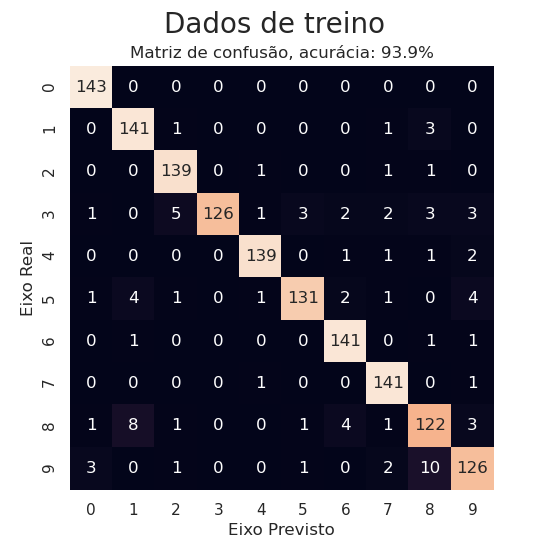
\includegraphics[width=10cm]{figuras/mnist_treino}
\caption{Matriz de confusão, função de perda e acurácia do conjunto de treino da base MNIST $8\times8$.}
\label{fig:mnist_treino}
\end{figure}

\begin{figure}[htb]
\centering
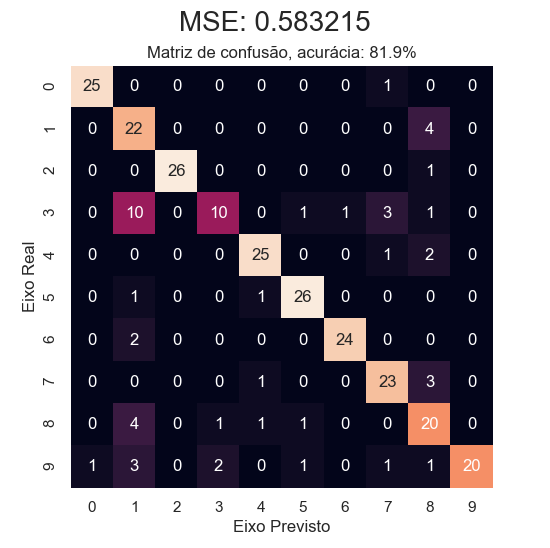
\includegraphics[width=10cm]{figuras/mnist_test}
\caption{Matriz de confusão, função de perda e acurácia do conjunto de teste da base MNIST $8\times8$.}
\label{fig:mnist_test}
\end{figure}

Como os pesos da rede são inicializados aleatoriamente, cada treinamento pode obter resultados levemente diferentes, embora que, no geral os resultados irão convergir para um resultado médio, que dependem dos parâmetros utilizados, como a função de ativação, quantidade de camadas e de neurônios e de épocas de treinamento.

Podemos notar que o conjunto de treino possui uma boa perfomance, obtendo mais de $93\%$ de acurácia, ou seja, de classificações corretas. Por outro lado, o conjunto de treino obteve apenas pouco mais de $81\%$, o que indica o problema de \eng{overfitting} em nossa rede, quando a classificação do treino está boa, o que é esperado dado que é a base utilizada para o ajuste dos parâmetros internos, mas quando a rede treinada tenta lidar com dados inéditos, o que é o papel do conjunto de teste, se sai consideravelmente pior.

Está demonstrada a necessidade da utilização de alguma implementação mais robusta, e refinada com anos de contribuições da comunidade de programadores e cientistas de dados ao redor do planeta. E essa implementação, ou pelo menos uma delas, é a API Keras, que veremos na próxima seção, e que será utilizada no restante desse trabalho.

\section{Utilizando a API Keras}

De acordo com seu site oficial\footnote{\url{https://keras.io/about/}}, \eng{Keras} é uma API (Interface de Programação de Aplicativos) de \eng{deep learning} escrita em Python, e que roda sobre a plataforma de \emph{deep learning} chamada de \eng{TensorFlow}\footnote{\url{https://www.tensorflow.org/}} que é de fato a biblioteca que devemos instalar em nosso ambiente Python, para podermos utilizar as redes neurais ali implementadas e quaisquer outros recursos da API \eng{Keras} em nosso projeto de aprendizado.

Keras implementa quase todas as arquiteturas de redes neurais, segundo Géron \citep{hands}, sua popularidade é devido sua facilidade de uso, flexibilidade aliadas a um lindo design de software. Existem algumas implementações da API, como a \emph{TensorFlow}, que é a principal, a \eng{Microsoft Cognitive Toolkit}, a \eng{Apache MXNet}, a \eng{Apple's Core ML}, etc. 

Todas essas implementações podem ser utilizadas em conjunto, na biblioteca conhecida como \eng{multibackend Keras}, sendo que a escolha entre uma delas ocorre de forma encapsulada até mesmo para o cientista de dados. Alternativamente, utilizar a versão própria presente na biblioteca \eng{TensorFlow} traz benefícios como recursos exclusivos à ela. O funcionamento dessas 2 implementações está na Figura \ref{fig:tensor_flow}, a seguir.

\begin{figure}[htb]
\centering
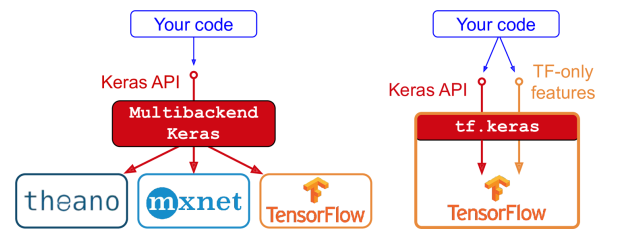
\includegraphics[width=12cm]{figuras/tensor_flow}
\caption{As 2 implementações da API Keras. \eng{Multibackend} à esquerda e \eng{TensorFlow} à direita.\footnote{Extraído de: Aurélien Géron, `Hands-on Machine Learning with Scikit-Learn, Keras, and TensorFlow', O'Reilly 2.a edição 2019, página 385.}}
\label{fig:tensor_flow}
\end{figure}

Para entender o funcionamento e uso do Keras, criei uma rede com a mesma estrutura do Perceptron aqui implementado mas com algumas melhorias já disponíveis com a API, e com objetivo de classificar o mesmo conjunto de dados MNIST, só que agora com a versão oficial da base de dados, o que é possível já que a biblioteca está implementada com muita eficiência e funciona bem para bases maiores mesmo num ambiente pessoal de computação. 

A importação da base é feita agora usando outra função da biblioteca \emph{sklearn}. Pode ser visto na listagem \ref{lst:keras_1}. A seguir os dados são divididos entre os conjuntos de treino e de teste, com as listas \texttt{x\_train, x\_test} e \texttt{y\_train, y\_test} contendo os pixels e as classficações respectivamente, como antes.

\begin{scriptsize}
\estiloR
\begin{lstlisting}[caption={Trecho do script \eng{mnist\_keras.py}}, label={lst:keras_1}, escapeinside={\%}]
from sklearn.datasets import fetch_openml
mnist = fetch_openml('mnist_784', version=1) # versao 28x28
\end{lstlisting}
\end{scriptsize}

O próximo passo é criar a rede utilizando a API Keras, o que vemos na listagem \ref{lst:keras_2}. A primeira linha cria uma rede sequencial, isto é, uma rede \eng{feedforward}. A seguir, são adicionadas as camadas, a primeira camada é definida como \eng{Flatten} pois é a camada de entrada, então ela não aplica nenhuma transformação nos dados. A base de dados é importada num formato matricial de $28\times28$ pixels, o que pode ser utilizado e tratado diretamente pela API.

\begin{scriptsize}
\estiloR
\begin{lstlisting}[caption={Trecho do script \eng{mnist\_keras.py}}, label={lst:keras_2}, escapeinside={\%}]
model = tf.keras.Sequential()
layers = tf.keras.layers

model.add(layers.Flatten(input_shape=(28, 28)))
model.add(layers.Dense(512, activation='elu'))
model.add(layers.Dense(256, activation='elu'))
model.add(layers.Dense(128, activation='elu'))
model.add(layers.Dense(10, activation='softmax'))

model.compile(optimizer=keras.optimizers.SGD(lr=0.001),
              loss='sparse_categorical_crossentropy', metrics=['accuracy'])
\end{lstlisting}
\end{scriptsize}

As próximas camadas são adicionadas com o tipo \eng{Dense}, o que significa uma conexão de todos os neurônios de uma camada com todos da próxima, dessa forma estamos criando um \eng{Perceptron} exatamente como aquele implementado. As camadas ocultas utilizam a função de ativação \eng{ELU}, e a camada de saída utiliza a função \eng{softmax}, o que na API Keras significa que estamos classificando os dados de acordo com o valor máximo dos neurônios de saída, o que em nossa implementação foi papel da função \texttt{reinterpretar\_saidas}, que foi definida na listagem \ref{lst:percep_6}.

Na última linha da listagem \ref{lst:keras_2}, definimos os parâmetros finais da rede. Define-se a função de otimização \eng{SGD} (\eng{Stocastic Gradient Descent}), quase idêntico à implementação do gradiente descendente implementada, mas ao invês de utilizar sempre todos os dados de treino numa época de treinamento, alguns são escolhidos aleatoriamente, e isso é feito um certo número de vezes, e os deltas são escolhidos para o conjunto aleatorio que tenha se saído melhor, de acordo com a função de perda e métrica utilizada.

A função de perda é escolhida com a opção \eng{sparse\_categorical\_crossentropy}, o que significa que a API irá tratar as categorias de dados da forma que ela foi obtida, com as $10$ classes de $0$ a $9$, onde cada imagem pertence a apenas uma dessas classes. Esse parâmetro seria diferente se fosse criada uma rede para classificação binária, por exemplo, ou então se nossos vetores \texttt{y\_train} e \texttt{y\_test} tivessem sido codificados em vetores do tipo $[0,\ldots,1,0,\ldots]$ da forma que foi feita na nossa implementação.

Por fim a acurácia é escolhida como a métrica para avaliação da rede, e que será utilizada pelo gradiente estocástico para definir o melhor sub-conjunto de treino durante uma dada época de treinamento. Basta treinar a rede como o método \eng{fit}, especificando o número de épocas de treinamento desejado, neste caso $15$ foram suficientes, o que está feito na listagem \ref{lst:keras_3}.

\begin{scriptsize}
\estiloR
\begin{lstlisting}[caption={Trecho do script \eng{mnist\_keras.py}}, label={lst:keras_3}, escapeinside={\%}]
model.fit(x_train, y_train, epochs=15)

test_loss, test_acc = model.evaluate(x_train, y_train, verbose=2)
test_loss, test_acc = model.evaluate(x_test, y_test, verbose=2)
\end{lstlisting}
\end{scriptsize}

Nessa listagem também está a avaliação da rede, para o conjunto de treino e para o conjunto de teste. Os resultados obtidos após $15$ épocas de treinamento foram $99.9\%$ de acurácia para o conjunto de treino e $96.4\%$ para o conjunto de teste. Por fim podemos fazer previsões com a rede treinada, nesse caso a API possui o método \eng{predict} que irá retornar os valores da camada de saída, ou seja, as probabilidades de cada imagem pertencer à uma das $10$ classes informadas durante o treinamento.

\begin{scriptsize}
\estiloR
\begin{lstlisting}[caption={Trecho do script \eng{mnist\_keras.py}}, label={lst:keras_4}, escapeinside={\%}]
y_pred = np.argmax(model.predict(x), axis=-1)

# usando a minha propria classe de validação
# e que mostra a acuracia e a matriz de confusão
score = Scores(y_test, y_pred)
score.exibir_grafico("Dados de teste")
\end{lstlisting}
\end{scriptsize}

Na listagem \ref{lst:keras_4}, está a lógica de obter a classificação predita para o conjunto de teste, utliza a função \eng{argmax} para obter a classe que obteve a probabilidade máxima. E por fim exibe a matriz de confusão dessa predição, o que está na Figura \ref{fig:keras_test}.

\begin{figure}[htb]
\centering
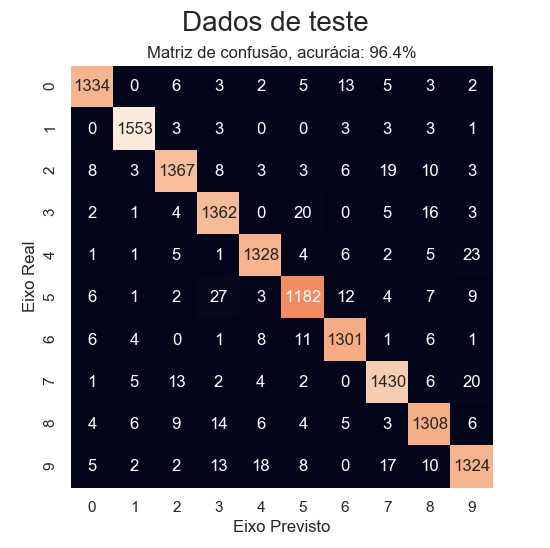
\includegraphics[width=10cm]{figuras/keras_test}
\caption{Matriz de confusão, função de perda e acurácia do conjunto de teste da base MNIST $28\times28$, utilizando a API Keras.}
\label{fig:keras_test}
\end{figure}

É notável a eficiência da API em comparação à nossa implementação simples. A rede é treinada em menos de $2$ minutos, mesmo sendo utilizada a base MNIST original que possui muito mais pixels e também muito mais imagens, $60$ mil em comparação às $2$ mil da base menor utilizada anteriormente. 

Além disso a acurácia final do conjunto de treino é praticamente perfeita, e o conjunto de treino, apesar de muito melhor em relação à implementação, ainda está relativamente menor à acurácia do treino, indicando que nessa versão imitada do \eng{Perceptron} existe o problema de \eng{overfitting}, mesmo que em menor intensidade.

É para resolver esse problema e outros, que existem diversas otimizações e configurações alternativas ao simples Perceptron, implementadas na API Keras. Existem várias outros métodos de otimização, outras funções de perda e sobretudo outras arquiteturas de rede que podem ser utilizadas em alternativa às camadas densas do perceptron. 

A estratégia utilizada no contexto de \eng{deep-learning} é sobretudo de tentativa e erro, e conforme um cientista de dados vai fazendo isso muitas vezes vai construindo conhecimentos sobre qual arquitetura usar para um problema, qual otimização funciona melhor, uma vez que isso irá sempre variar de acordo com a base de dados utilizada, seja para classificação seja para regressão.

Uma tentativa recente de melhora nessa estratégia foi a criação de uma biblioteca cujo objetivo é o de justamente testar entre diversas arquiteturas e demais parâmetros de criação de uma rede neural, qual a que se sairá melhor para um dado conjunto de dados e objetivo de aprendizagem. Essa biblioteca é chamada de \eng{AutoKeras} e pertence à essa nova vertente de \eng{deep-learning} conhecida como AutoML (\eng{Automated Machine Learning}).

Os objetivos da AutoML é, segundo Andre Ye \citep{automl}, é o de tornar \eng{deep-learning} mais acessível para o aprendizado de todos os entusiastas, e também o de acelerar o desenvolvimento de pesquisas nessa área, para tornar a criação de conhecimentos mais sólidos e gerar mais \eng{insigths} para a interpretabilidade dos modelos de redes neurais.

Em seu artigo, Andre Ye \citep{automl} demostra como instalar e utilizar o \eng{AutoKeras}. Resumidamente, o que fazemos é informá-la com a nossa base de dados, e ela irá fazer todo o trabalho de escolha da arquitetura e dos parâmetros, e ao final retornará um objeto da API Keras, que poderá ser usado tanto para tarefas de classificação quanto de regressão. 

Uma desvantagem a ser considerada é o tempo de processamento da biblioteca \eng{AutoKeras}. Dessa forma, para problemas de menor escala, tanto de quantidade de dados utilizada quanto de poder computacional disponível, o que inclui o que iremos fazer a seguir na previsão de séries temporais, é mais viável testar dentre alguns poucos parâmetros conhecidamente melhores a partir da experiência de outros cientistas de dados, o que implica num tempo consideravelmente menor de processamento.
